\documentclass[11pt, a4paper]{article}
\usepackage[margin=1in]{geometry}
\usepackage[hidelinks]{hyperref}
\usepackage{amsfonts, amssymb, amsmath}
\usepackage{enumerate}
\usepackage{float}
\usepackage{tikz}
% \usepackage{pgfplots}
% \usetikzlibrary{decorations.pathreplacing}



\title{
    \textbf{Math 401 Notes} \\
    Lecture 1\&2 \\ (Statistics)
}

\author{Ahmed Nasser}
\date{\today}


\begin{document}
    \maketitle
    \tableofcontents 
    \pagebreak

    \section{Statistics Steps}
    \begin{enumerate}
        \item Collect
        \item Organize
        \item Present
        \item Summarize
        \item Draw Conclusion
    \end{enumerate}

    \section{Types of Data}
    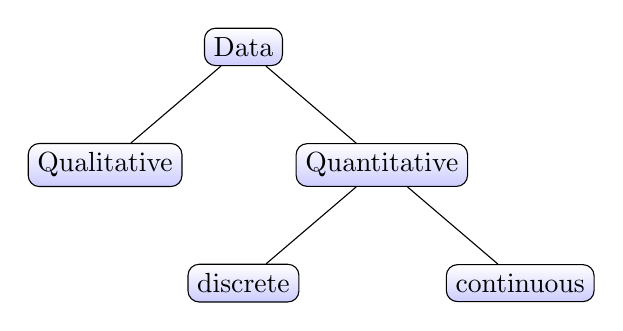
\begin{tikzpicture}[sibling distance=10em,
        every node/.style = {shape=rectangle, rounded corners,
          draw, align=center,
          top color=white, bottom color=blue!20}]]
        \node {Data}
          child { node {Qualitative} }
          child { node {Quantitative}
            child { node {discrete}}
            child { node {continuous} } };
      \end{tikzpicture}    

      \section{Types of statistical studies}
      \begin{enumerate}
          \item \textbf{Descriptive statistics}
          \subitem collecting, organizing,
          presenting, and summarizing of data, in
          an informative way.     
          \item \textbf{Inferential statistics}
          \subitem drawing conclusions and making
          decisions using the given data 
      \end{enumerate}

      \section{Present (Graphs)}
      \subsection{Histogram}
      \begin{itemize}
          \item $X$-axis -- Class Limits
          \item $Y$-axis -- “$f$” or “$r. f.$”
      \end{itemize}
      \subsection{Ogive}
      \begin{itemize}
        \item $X$-axis -- Upper limits of each class limit
        \item $Y$-axis -- “$c.f.$” or “$c.r. f.$”
    \end{itemize}


      \section{Range \& Width}
      \begin{enumerate}
          \item Range = Max Val - Min Val
          \item Class Width = $\displaystyle \frac{\text{Range}+1}{\text{No. of classes}}$  {\ \ \ \ \ \small If this value is not an integer ROUND IT UP}
      \end{enumerate}

     \section{ grouped frequency distribution}
     \begin{itemize}
         \item If the \textbf{number of classes is given} and the given data values are integers: we
         proceed using the \textbf{direct method}
         \item If the \textbf{number of classes is NOT given} and the given data values are integers
or decimals
        \subitem If an \textbf{initial value is NOT given}, we proceed using the \textbf{Stem-leaf method}.
        \subitem If an \textbf{initial value is given}, we proceed using the \textbf{(
            $\sqrt{n}$ ) method}. (Width = $\frac{\text{Range}}{\text{No. of classes}}$)
     \end{itemize}

     \section{The Median}

     \subsection{Discrete Data}
     \begin{itemize}
         \item Sort the Data value   
         \item MD = middle point  {\small (in case of odd num)}
         \item MD = (sum of the two middle points) / 2  {\small (in case of odd num)} 
     \end{itemize}

     \subsection{Grouped data}
     $$\text{MD} = \frac{\frac{n}{2} - \text{pre.}"c.f"}{f}(W)+L_m$$
     where $W$ is the class width and $L_m$ is the lower bound \\
     \textbf{ex:} if the median is 80 then about 50\% of student achieved more than 80 and 50\% achieved less than 80 

     \section{The Mode}
     \subsection{Discrete Data}
     \begin{itemize}
        \item The mode is a data value that has the highest frequency in a data set
        \item If all of data values have the same frequency then there is no mode
          
     \end{itemize}
     \subsection{Grouped data}
     \begin{itemize}
         \item We use Modal class instead of mode in grouped data 
         \item The modal class is the class corresponds to the highest frequency
     \end{itemize}


     \section{The Mean}
     \subsection{Discrete Data}
     \begin{itemize}
         \item For a population
         $$\displaystyle \mu = \frac{\sum_{i = 1}^{N} X_i}{N}$$
         \item For a Sample
         $$\displaystyle \bar{X} = \frac{\sum_{i = 1}^{n} X_i}{n}$$
     \end{itemize}

     \subsection{Grouped data}
     $$\mu = \frac{\sum f.X_m}{\sum f}=\frac{\sum f.X_m}{N} $$
     Where $X_m$ is the class midpoint

     \subsection{Weighted data}
     $$\mu = \frac{\sum_{i = 1}^{n} W_iX_i}{\sum_{i = 1}^{n} W_i}$$

     \section{The Standard Deviation}
     \begin{itemize}
        \item For a population
        $$\sigma := \sqrt{\sigma^2}$$
        \item For a Sample
        $$S := \sqrt{S^2}$$
    \end{itemize}

    \section{The Population Variance}
    \subsection{Discrete Data}
    \begin{itemize}
        \item For a population
        $$\sigma^2 = \frac{\sum_{i=1}^N (X_i-\mu)^2}{N}$$
        \item For a Sample
        $$S^2 = \frac{\sum_{i=1}^n (X_i-\bar{X})^2}{n-1}$$
        $$S^2 = \frac{\sum_{i=1}^n X_i^2-\frac{\left(\sum_{i=1}^nX_i\right)^2}{n}}{n-1}$$

    \end{itemize}

    \subsection{Grouped data}
    \begin{itemize}
        \item For a population
        $$\sigma^2 = \frac{\sum f.(X_m-\mu)^2}{\sum f}$$
        \item For a Sample
        $$S^2 = \frac{\sum f.X_m^2-\frac{\left(\sum f.X_m\right)^2}{\sum f}}{\left(\sum f\right)-1}$$

    \end{itemize}

    \section{Chebyshev’s Theorem}
    $[\bar{x}-ks,\bar{x}+ks]$ is the smallest interval thant contains at least $\left(1-\frac{1}{k^2}\right)*100\%$ of the data

    \section{Percentiles}
    \begin{itemize}
        \item Sort your data values 
        $$\text{Percentile} = \frac{0.5 + \text{No. of values below }X}{n}*100\% $$
        \item $n$ is number of data and $p$ is the percentile then evaluate m = $n.p$
        \subitem if $m$ is not integer round it up and then $p$ corresponds \textbf{data value}[m]
        \subitem if $m$ is integer then $p$ corresponds the average of \textbf{data value}[m] and \textbf{data value}[m+1]
    \end{itemize}

    \section{Quartiles}
    \begin{itemize}
     \item $Q_1 = 25^{\text{th}}$ percentile
     \item $Q_2 = 50^{\text{th}}$ percentile |or| median
     \item $Q_3 = 75^{\text{th}}$ percentile
    \end{itemize}
\end{document}
